\documentclass[
	12pt,				
	openright,		
	twoside,	
	a4paper,
	english,	
	brazil	
	]{abntex2}
\usepackage{lmodern}		
\usepackage[T1]{fontenc}	
\usepackage[utf8]{inputenc}
\usepackage{lastpage}	
\usepackage{indentfirst}
\usepackage{color}	
\usepackage{graphicx}
\usepackage{microtype}
\graphicspath{{./imagens/}}
\usepackage{lipsum}			
\usepackage[brazilian,hyperpageref]{backref}	 
\usepackage[alf]{abntex2cite}	
\renewcommand{\backrefpagesname}{Citado na(s) página(s):~}
\renewcommand{\backref}{}
\renewcommand*{\backrefalt}[4]{
	\ifcase #1 %
		Nenhuma citação no texto.%
	\or
		Citado na página #2.%
	\else
		Citado #1 vezes nas páginas #2.%
	\fi}%
\titulo{Análise de IDPSs}
\autor{Glenon Mateus Barbosa Araújo}
\local{Brasil}
\data{\the\year}
\orientador{Dr. Roberto Samarone dos Santos Araújo}
%\coorientador{}
\instituicao{
  Universidade Federal do Pará -- UFPA
  \par
  Faculdade de Computação
  \par
  Bacharelado em Ciência da Computação}
\tipotrabalho{Trabalho de Conclusão de Curso}
\preambulo{Trabalho de Conclusão de Curso submetida a graduação em Ciência da Computação da UFPA}
\definecolor{blue}{RGB}{41,5,195}
\makeatletter
\hypersetup{
     	%pagebackref=true,
		pdftitle={\@title}, 
		pdfauthor={\@author},
    	pdfsubject={\imprimirpreambulo},
	    pdfcreator={LaTeX with abnTeX2},
		pdfkeywords={abnt}{latex}{abntex}{abntex2}{trabalho acadêmico}, 
		colorlinks=true,       	
    	linkcolor=blue,          
    	citecolor=blue,        	
    	filecolor=magenta,     
		urlcolor=blue,
		bookmarksdepth=4
}
\makeatother
\setlength{\parindent}{1.3cm}
\setlength{\parskip}{0.2cm} 
\makeindex
\begin{document}
\selectlanguage{brazil}
\frenchspacing 
\imprimircapa
\imprimirfolhaderosto*
\begin{fichacatalografica}
	\sffamily
	\vspace*{\fill}
	\begin{center}
	\fbox{\begin{minipage}[c][8cm]{13.5cm}	
	\small
	\imprimirautor
	\hspace{0.5cm} \imprimirtitulo  / \imprimirautor. --
	\imprimirlocal, \imprimirdata-
	\hspace{0.5cm} \pageref{LastPage} p. : il. (algumas color.) ; 30 cm.\\
	\hspace{0.5cm} \imprimirorientadorRotulo~\imprimirorientador\\
	\hspace{0.5cm}
	\parbox[t]{\textwidth}{\imprimirtipotrabalho~--~\imprimirinstituicao,
	\imprimirdata.}\\
	\hspace{0.5cm}
		1. Suricata.
		2. Snort.
		3. IDPS.
		I. Orientador.
		II. Universidade Federal do Pará.
		III. Faculdade de Computação.
		IV. Análise de IDPSs
	\end{minipage}}
	\end{center}
\end{fichacatalografica}
\begin{errata}
Elemento opcional da \citeonline[4.2.1.2]{NBR14724:2011}. Exemplo:
\vspace{\onelineskip}
FERRIGNO, C. R. A. \textbf{Tratamento de neoplasias ósseas apendiculares com
reimplantação de enxerto ósseo autólogo autoclavado associado ao plasma
rico em plaquetas}: estudo crítico na cirurgia de preservação de membro em
cães. 2011. 128 f. Tese (Livre-Docência) - Faculdade de Medicina Veterinária e
Zootecnia, Universidade de São Paulo, São Paulo, 2011.
\begin{table}[htb]
\center
\footnotesize
\begin{tabular}{|p{1.4cm}|p{1cm}|p{3cm}|p{3cm}|}
  \hline
   \textbf{Folha} & \textbf{Linha}  & \textbf{Onde se lê}  & \textbf{Leia-se}  \\
    \hline
    1 & 10 & auto-conclavo & autoconclavo\\
   \hline
\end{tabular}
\end{table}
\end{errata}
\begin{folhadeaprovacao}
  \begin{center}
    {\ABNTEXchapterfont\large\imprimirautor}
    \vspace*{\fill}\vspace*{\fill}
    \begin{center}
      \ABNTEXchapterfont\bfseries\Large\imprimirtitulo
    \end{center}
    \vspace*{\fill}
    
    \hspace{.45\textwidth}
    \begin{minipage}{.5\textwidth}
        \imprimirpreambulo
    \end{minipage}%
    \vspace*{\fill}
   \end{center}
        
   Trabalho aprovado. \imprimirlocal, 24 de novembro de 2012:
   \assinatura{\textbf{\imprimirorientador} \\ Orientador} 
   %\assinatura{\textbf{Professor} \\ Convidado 1}
   %\assinatura{\textbf{Professor} \\ Convidado 2}
   %\assinatura{\textbf{Professor} \\ Convidado 3}
   %\assinatura{\textbf{Professor} \\ Convidado 4}
      
   \begin{center}
    \vspace*{0.5cm}
    {\large\imprimirlocal}
    \par
    {\large\imprimirdata}
    \vspace*{1cm}
  \end{center}
  
\end{folhadeaprovacao}
\begin{dedicatoria}
   \vspace*{\fill}
   \centering
   \noindent
   \textit{•} \vspace*{\fill}
\end{dedicatoria}
\begin{agradecimentos}
\end{agradecimentos}
\begin{epigrafe}
    \vspace*{\fill}
	\begin{flushright}
		\textit{•}
	\end{flushright}
\end{epigrafe}
\setlength{\absparsep}{18pt} 
\begin{resumo}
 \textbf{Palavras-chave}: Segurança, Suricata, Snort, Sistema de Detecção de Intrusão, Sistema de Prevenção de Intrusão, IDS, IPS.
\end{resumo}
\begin{resumo}[Abstract]
 \begin{otherlanguage*}{english}
   \vspace{\onelineskip}
 
   \noindent 
   \textbf{Keywords}: Security, Suricata, Snort, Intrusion Detection System, Intrusion Prevention System, IDS, IPS.
 \end{otherlanguage*}
\end{resumo}
\pdfbookmark[0]{\listfigurename}{lof}
\listoffigures*
\cleardoublepage
\pdfbookmark[0]{\listtablename}{lot}
\listoftables*
\cleardoublepage
\begin{siglas}
  \item[IDS] \textit{Intrusion Detection System}
  \item[IPS] \textit{Intrusion Prevention System}
  \item[MB] \textit{Megabytes}
  \item[GB] \textit{Gigabytes}
  \item[SO] \textit{Sistema Operacional}
  \item[JSON] \textit{JavaScript Object Notation}
\end{siglas}
\pdfbookmark[0]{\contentsname}{toc}
\tableofcontents*
\cleardoublepage
\textual
\chapter*[Introdução]{Introdução}
\addcontentsline{toc}{chapter}{Introdução}
\section*{Objetivos}
\section*{Trabalhos Relacionados}
\section*{Motivação}
\chapter{Segurança de Redes de Computadores}
\section{Cenário Geral}
\section{Ataques}
\subsection{Varredura de Redes}
\subsection{Exploração de Vulnerabilidades}
\subsection{Força Bruta}
\subsection{Desfiguração de páginas}
\subsection{Negação de Serviços}
\subsection{Worm}
\subsection{Trojan}
\subsection{Fraudes - Direitos Autorais}
\chapter{Sistemas de Detecção e Prevenção de Intrusão}
\section{Tipos de IDS/IPS}
\section{Snort}
\section{Suricata}

\chapter{Detecção de Intrusão em um Cenário Real}
%- Em cada capitulo adicionar um texto introdutório

Este capítulo esta organizado da seguinte forma: A próxima seção apresenta o cenário de testes, descrevendo características gerais da rede selecionada para os teste. Na seção \ref{sec:infraestrutura} será abordado a infraestrutura usada para os testes, ferramentas utilizadas e as configurações feitas. Na seção \ref{sec:testes} será descrito os testes realizados com suas respectivas justificativas. Na seção \ref{sec:resultados} será apresentado os resultados esperados e obtidos, problemas encontrados e a comparação das ferramentas e por último, na seção \ref{sec:conclusão}, uma breve conclusão.

\section{Cenário de Testes} \label{sec:cenário}
%Descrever o cenário. Ex: Uma rede com XXX usuários; Os usuários utilizam
%diferentes ferramentas,...
%Adicionar gráficos de utilização da rede

A rede selecionada para ser monitorada tem os valores especificados na tabela. Podemos verificar que em um determinado período do dia o pico de trafego chega a 107,25 Mbps, valores considerados ideais para o experimento, inclusive para tentar validar os recursos alocados. Figura \ref{fig:ilc}

Em um primeiro momento, selecionou-se uma rede

\begin{figure}[!htp]
 \centering
 \includegraphics[scale=.6]{ILC-editado.png}
 \caption{Estatística da rede usada para os testes}
 \label{fig:ilc}
\end{figure}

\section{Infraestrutura definida para testes} \label{sec:infraestrutura}
%Descrever o que foi utilizado:
%Ex: Equipamentos - Servidores, ....
%    Configuração
%    Ferramentas - Snort (referenciar capítulo), ...

No ambiente de teste foi usado uma máquina Dell com 134 Megabytes (MB) de memória RAM e 40 núcleos. Usou-se XenServer \cite{xenserver} versão 7, sistema operacional (SO) \textit{opensource} da Citrix voltado para virtualização. Foram testados outros SOs porém somente o XenServer possuía, na época da instalação do ambiente, \textit{firmware} da placa de rede do \textit{host} compatível e que funcionava com instabilidade. Outro fator que pesou na escolha do SO foi a experiência que tinha com a plataforma e por existir uma interface para gerencia chamada XenCenter que roda no Windows. Uma alternativa \textit{opensource} desse software é o OpenXenManager \cite{openxenmanager}.

No primeiro momento, foi instalado uma máquina virtual com o sistema operacional Debian 7.11 \textit{codename} Wheezy \cite{debianwheezy}, uma distribuição linux com uma proposta de ser totalmente livre, usada como base para instalação de outras máquinas utilizando o recurso de \textit{snapshot}, uma cópia de uma máquina virtual rodando em um certo momento, do XenServer. O uso desse recurso foi necessário para criar um ambiente igual para os IDSs.

Foi alocado 8 MB memória RAM, 4 processadores e 100 Gigabytes(GB) de espaço em disco para o \textit{snapshot}. Esses valores foram definidos com base em um estudo \cite{mikelococo} que considerava vários fatores, como largura da rede, localização do IDS e versão e tipo do capturador de tráfego para dimensionar os recursos, aplicado especificamente ao Snort. A mesma regra foi aplicada ao Suricata.

Para o \textit{host} conseguir pegar o pacotes destinados a rede selecionada foi necessário uma configuração de espelhamento que consiste na copia dos pacotes que saem pela porta dessa rede no \textit{switch} para a porta conectada no \textit{host}. A interface de rede do \textit{host} precisou ser configurado no modo \textit{promisc}.

Posteriormente criou-se três máquinas virtuais, duas usadas para instalação dos IDSs (Suricata e Snort) e a terceira para instalação das ferramentas usadas para simular ataques a rede. Optou-se pela instalação do sistema Kali \cite{kalilinux} para geração de ataques pois nele existe várias ferramentas nativas para testes de penetração e auditoria de segurança. A infraestrutura pode ser visualizada na Figura \ref{fig:infra-ambiente}.

Para coleta das informações de uso de recurso de hardware como memória, processamento e I/O das máquinas com os IDSs foi usado o \textit{daemon} Collectd \cite{collectd}. Outra opção para esse fim é a utilização de um servidor de monitoramento com o Zabbix \cite{zabbix}. A ideia de usar duas ferramentas para analise é fazer um comparativo e validar as informações coletadas.

O formato usado para facilitar a análise do \textit{logs} foi JavaScript Object Notation (JSON), um formato simples, leve e de fácil leitura. O Motor de Saída do Suricata já tem suporte a esse tipo de formato o que não acontece no Snort. Para tal, usou-se o IDSTools \cite{py-idstools}, uma coleção de bibliotecas na linguagem \textit{python} que trabalha para auxiliar o IDS, compatível com as ferramentas estudas. Dentre os utilitários presentes nessa coleção, temos o idstools-u2json, que converte, de forma continua, arquivo no formato unified2, uma das saídas disponível no Snort, para o formato JSON.

Para analisar os \textit{logs}

\begin{figure}[!htp]
 \centering
 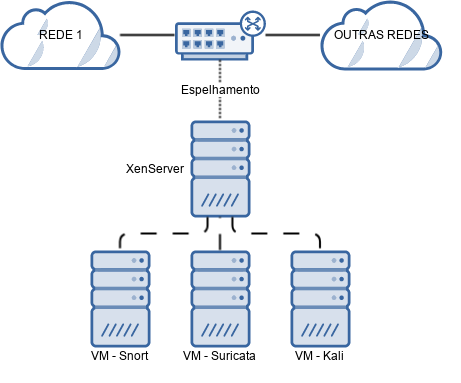
\includegraphics[scale=.6]{infra.png}
 \caption{Infraestrutura do ambiente de teste}
 \label{fig:infra-ambiente}
\end{figure}

\section{Testes Realizados} \label{sec:testes}
%Quais os testes realizados com justificativa ?
%Descrição dos testes. Quais os testes foram realizados ?
\subsection{NMAP} \label{sec:nmap}
\subsection{Pytbull} \label{sec:pytbull}
\subsection{Metasploit Framework} \label{sec:metasploit}
\section{Resultados} \label{sec:resultados}
%Resultados esperados e obtidos
%Quais os resultados dos testes ??
%Comparação das ferramentas
%Problemas encontrados
\section{Conclusão} \label{sec:conclusão}
\section{Métricas de Comparação}
%Consumo dos Recursos de Hardware (Memória, Processamento)
%Taxa de Detecção
%Número de Falsos Positivos/Negativos
\chapter{Considerações Finais} \label{considerações}
\phantompart
\postextual
\bibliography{bib/dissertacao}
\phantompart
\printindex
\end{document}
